\section{MAAS}\label{subsec:maas}

MAAS (Metal-as-a-Service \cite{maas_home}) è uno strumento open source e gratuito di provisioning di server e di host bare-metal creato e mantenuto da Canonical.
%
Ha come compito quello di aiutare, facilitare e automatizzare l'implementazione e il provisioning dinamico su ambienti di elaborazione iperscalabili (hyperscale computing enviroments) come cloud service o big data workloads.
% 
Per fare questo, MAAS collabora con diversi servizi come Juju per coordinare applicazioni e carico di lavoro, riuscendo così a distribuire hardware e servizi che possono scalare dinamicamente verso l'alto e verso il basso.

Permette quindi il monitoraggio e il rilevamento automatico dell'infrastruttura, la creazione di cloud bare metal con server on-demand, il deploy automatizzato di immagini anche con applicazioni preinstallate, la configurazione completa della rete e dello storage e il testing e commissioning dell'hardware.



\subsection{Funzionamento: i Controller}
Il funzionamento di MAAS è suddiviso in due tipi di controller: un singolo region controller (regiond) e uno o più rack controller (rackd).
% 
Nell'esempio riportato in \cref{fig:maas_controllers} viene mostrato uno scenario dove il region controller gestisce due rack controller.

\paragraph{Region Controller.}
Il region controller è il cuore di MAAS; gestisce i rack controller fornendo loro le immagini da utilizzare per il provisioning delle macchine. Utilizza un database PostgreSQL per mantenere lo stato dei nodi registrati al sistema e ospita alcuni dei servizi di rete principali, come ad esempio il server DNS o il proxy HTTP.
%
Inoltre comunica con l'utente attraverso un'interfaccia web e una serie di API REST, dalle quali è possibile configurare e gestire tutto il sistema.

\paragraph{Rack Controller.}
 Il rack controller gestisce effettivamente le macchine collegate al sistema, occupandosi del deploy delle immagini fornite dal region controller.
 %
Gestisce la rete delle macchine, fornendo servizi come DHCP per l'assegnamento degli indirizzi IP, PXE per rendere possibile l'avvio da rete, TFTP per il trasferimento file, etc.
%
Vengono chiamati rack controller perché idealmente gestiscono individualmente singoli armadi rack con le relative macchine.
% 
Inoltre ogni rack controller è collegato via rete ad un "fabric" (vedasi la \cref{subsubsec:maas_rete} per maggior dettagli).
% 
\begin{figure}[H]
    \centering
    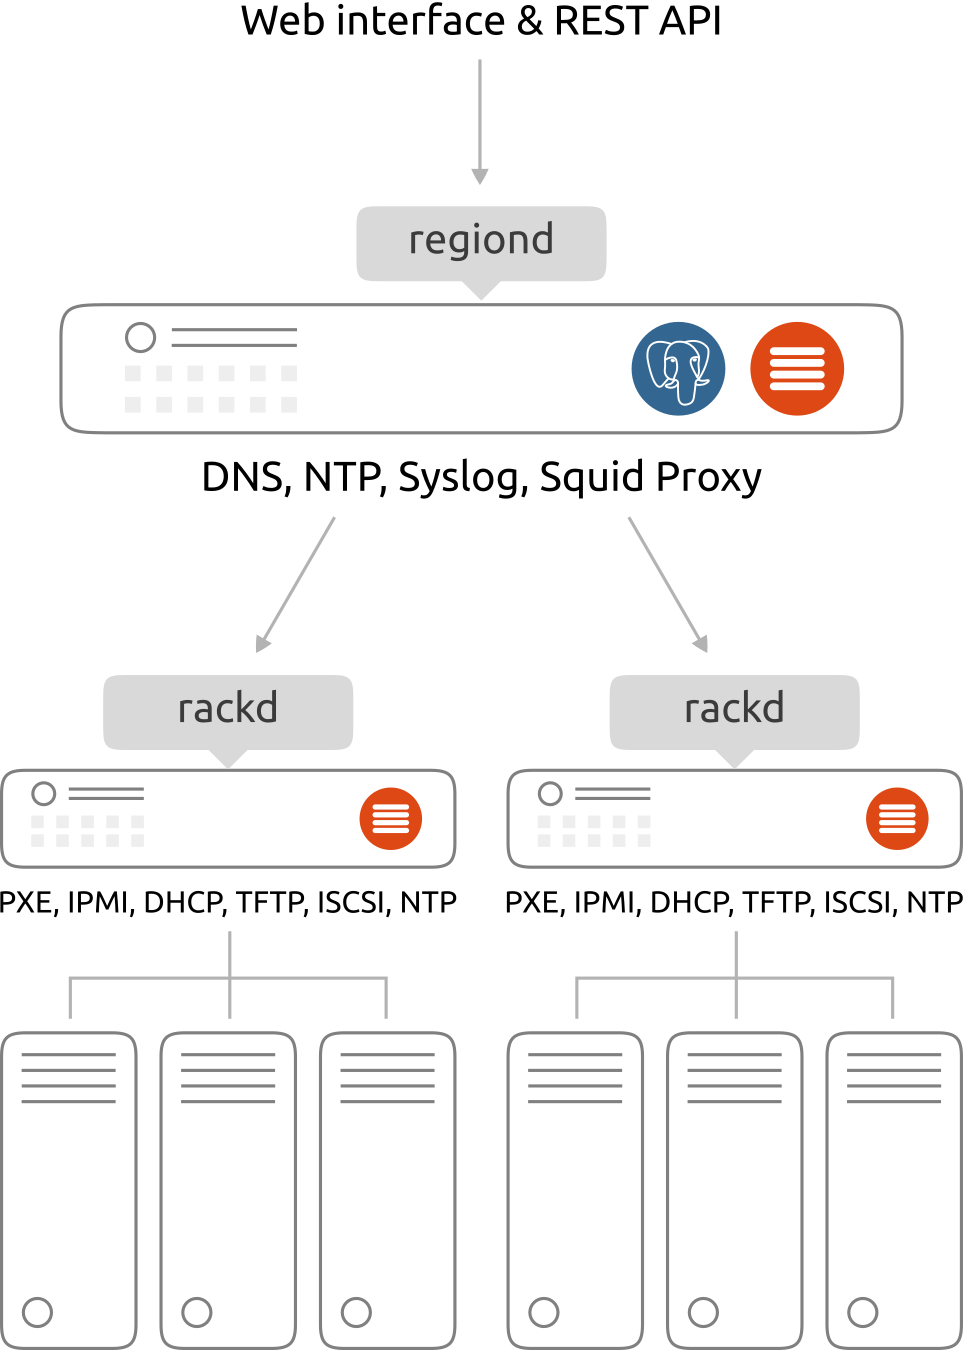
\includegraphics[width=0.45\linewidth]{tesi/files/immagini/maas/controllers}
    \caption{Configurazione con un region controller (regiond) e due rack controller (rackd) \cite{maas_how_it_works}.}
    \label{fig:maas_controllers}
\end{figure}

% \paragraph{}
% \bigskip
\noindent
Per un sistema di piccole dimensioni è possibile collocare sia il region controller che il rack controller sulla stessa macchina.\label{ref:region+rack}
%
Durante lo svolgimento di questa tesi è stato scelto questo approccio, in quanto trattasi di un piccolo scenario di prova del sistema.



\subsection{Risorse: i Nodi}\label{subsubsec:maas_node}
I nodi sono gli oggetti registrati su MAAS e ve ne sono di tre tipi:
\begin{itemize}
    \item \emph{Controllers}: sono i nodi che assumono il ruolo di region controller e rack controller.

    \item \emph{Machines}: sono i nodi che vengono gestiti tramite MAAS, ovvero quelli il cui deployment è gestito da MAAS.

    \item \emph{Devices}: sono altri dispositivi collegati alla rete che non vengono gestiti da MAAS ma che sono stati rilevati, come ad esempio router.
\end{itemize}
%
Ad ogni \textit{machine} è associata un etichetta che ne identifica lo stato attuale del lifecycle.
% 
I principali stati del lifecycle di una machine sono:
\begin{itemize}
    \item \emph{New}:
    quando una nuova risorsa viene collegata alla rete del rack controller, MAAS la rileva in automatico (fase di enlist);
    % 
    quindi l'aggiunge, registra il suo indirizzo MAC e gli associa lo stato \emph{New}.

    \item \emph{Commissioning}: è la fase durante la quale vengono raccolte e registrate le informazioni sulla configurazione dell'hardware della macchina, come quantità di RAM, numero di CPU, spazio sui dischi e altri device presenti sulla macchina stessa (e.g. GPU).

    \item \emph{Ready}: una volta terminata con successo la fase di \emph{Commissioning}, lo stato della macchina viene modificato in \emph{Ready}.

    \item \emph{Allocated}: questo stato indica che una macchina in \emph{Ready} è stata allocata ad un utente ed è pronta per il deploy.

    \item \emph{Deploying}: durante questa fase viene installato il sistema operativo in maniera completamente automatica, applicando le varie configurazioni che sono state scelte.

    \item \emph{Deployed}: è lo stato che identifica una macchina come utilizzata, ovvero con il sistema operativo installato e in funzione.

    \item \emph{Releasing}: se una macchina non è più necessaria è possibile eseguire il \textit{release}, ovvero rilasciarla in modo che possa essere riutilizzata per altri scopi. 
    % 
    Durante questa fase è possibile cancellare i dati dei dischi, scegliendo il grado di profondità dell'operazione.
    %se una macchina non è più necessaria, è possibile rilasciarla nell’insieme delle macchine Ready. 
    %
    % In questa fase è possibile cancellare i dati dei dischi, scegliendo il grado di profondità dell'operazione.
\end{itemize}
% 
Oltre a questi, esistono altri stati che permettono di identificare il malfunzionamento dei nodi o di un’azione intrapresa su di essi, come ad esempio \emph{Failed testing}, \emph{Failed Commissioning}, \emph{Failed Deployment}, \emph{Broken}, \emph{Locked}, etc.



\subsection{Gestione della rete} \label{subsubsec:maas_rete}
%
Una corretta gestione della rete di provisioning è un punto cruciale per il corretto funzionamento di MAAS.
% 
La rete viene gestita da MAAS tramite l'uso di \emph{fabric} e di \emph{space}.
% MAAS gestisce la rete tramite l'uso di \emph{fabric} e di \emph{space}.
\paragraph{Fabric.} Il fabric concettualmente corrisponde ad uno switch o ad una combinazione di switch che utilizzano il trunking (VLAN Trunking Protocol, VTP \cite{vtp}) per fornire accesso a specifiche VLAN (Virtual LAN).
%
Il fabric racchiude un insieme di VLAN, a cui appartengono le sottoreti, che possono anche essere controllate da MAAS; in questo modo si rende possibile la comunicazione tra le varie VLAN appartenenti allo stesso fabric 
% e ciò permette a MAAS di fungere anche da server DHCP.
e ciò permette a MAAS di ricoprire anche il ruolo di server DHCP.

% \sout{Infatti, per poterli gestire a pieno ha bisogno di aver completo controllo della subnet su cui sono collegate le macchine nei rack, agendo così da gateway e da server DHCP.}
In una sottorete gestita in questo modo da MAAS è possibile amministrare gli indirizzi IP sia per riservarne un pool per usi diversi dal provisioning degli host, sia per gestirli dinamicamente per usarli e associarli automaticamente durante l'enlist, commission e deploy dei nodi.
% In una sottorete gestita in questo modo da MAAS è possibile amministrare gli indirizzi IP sia riservandone un pool per allocarli per usi diversi dal provisioning degli host, sia gestirli dinamicamente per usarli e associarli automaticamente durante l'enlisting, commisisioning e deploy dei nodi.
% In una sottorete così gestita da MAAS è possibile riservare un pool di indirizzi IP ed ad allocarli per usi diversi dal provisioning degli host, mentre riservando dinamicamente gli indirizzi IP, questi vengono associati durante l'enlisting, commisisioning e deploy dei nodi.

\paragraph{Space.} 
% Uno space è un raggruppamento logico di sottoreti 
% % in base a vari parametri
% , permettendone così la comunicazione diretta tra esse.
%
Le sottoreti possono essere raggruppate tra loro anche se appartengono a fabric differenti.
% 
In questi raggruppamenti, gli space, le sottoreti possono comunicare direttamente tra loro.
% 
Ciò è utile in caso si desideri separare i nodi in base all'utilizzo o per motivi di sicurezza.
% 
Ogni space ha un indirizzo IP e una subnet mask, e i nodi assegnati ad esso possono comunicare tra loro attraverso questa rete logica.
 
Un uso comune è lo space DMZ, usato per raggruppare le sottoreti che espongono un'interfaccia web verso la rete internet pubblica; dietro questa DMZ si possono trovare ad esempio le applicazioni che non possono interagire direttamente con l'utente ma che devono invece interagire con un'interfaccia Web all'interno dello space DMZ.
% 
Inoltre, gli space facilitano l'allocazione delle macchine per Juju.

% \bigskip
\vfill\break
\vfill\break
% \newpage
\noindent
Durante l'installazione, MAAS crea un fabric di default ("fabric-0", "fabric-1", etc) per ogni subnet rilevata, mentre non crea alcuno space.
% 
Nello scenario d'esempio di questo documento
verrà utilizzata la subnet \code{10.0.0.0/24} e dunque MAAS assocerà a questa il "fabric-0", mentre non è stato creato nessuno space in quanto non si è rilevato necessario.
% verrà utilizzato un fabric denominato "fabric-0" e nessuno space.

Il diagramma in \cref{fig:maas_fabric} mostra un esempio generico di data center contenente due fabric, ognuno delle quali contiene due rack controller, diverse VLAN e uno space in comune tra i due fabric.

\begin{figure}[H]
    \centering
    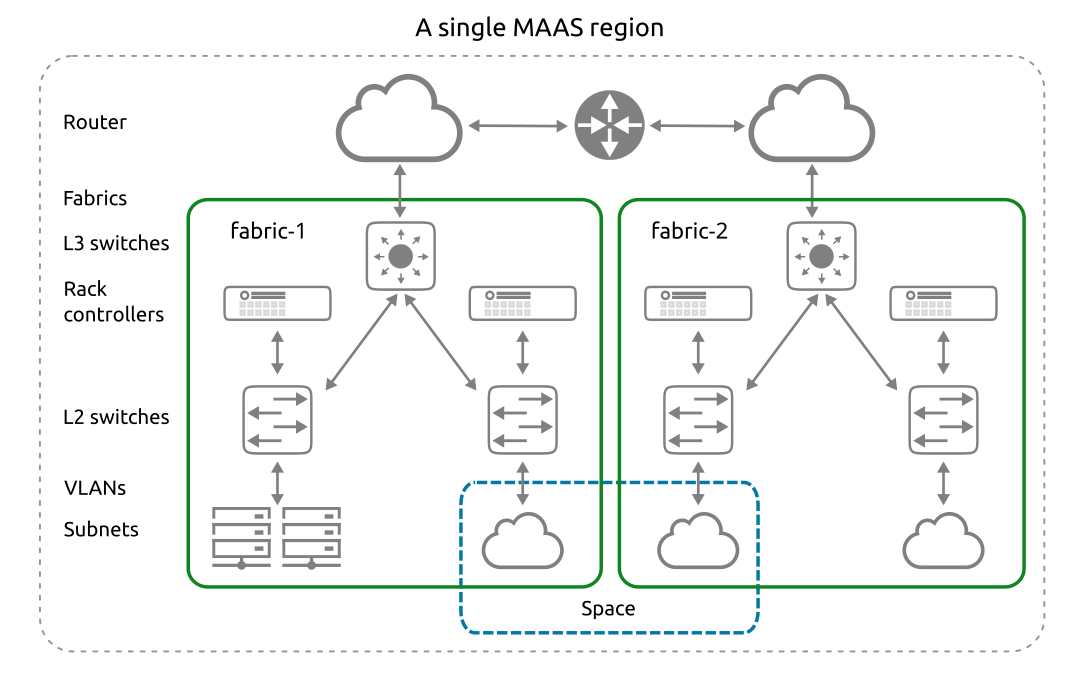
\includegraphics[width=1\linewidth]{tesi/files/immagini/maas/fabric}
    \caption{Esempio generico di configurazione di rete di un data center \cite{maas_glossary}.}
    \label{fig:maas_fabric}
\end{figure}



\subsection{Requisiti del sistema MAAS}
Il sistema che ospita MAAS non richiede un hardware eccessivamente prestante, tuttavia a seconda della configurazione finale i requisiti possono variare notevolmente.
%
Di seguito verranno mostrati due scenari d'esempio con i relativi requisiti di sistema stimati da Canonical \cite{maas_req}.


\bigskip
\paragraph{Test environment.}\label{sec:maas_req_test}
Questo è uno scenario proof-of-concept ed è l'ideale per testare e provare le potenzialità di MAAS prima di procedere con la vera e propria messa in produzione.
% 
È un tipo di scenario minimale, quindi non è necessario disporsi di macchine estremamente performanti.
% 
Nella \cref{tab:mass_requ_test} 
viene mostrata la stima delle risorse richieste da ogni componente per questo scenario.
% vengono mostrati i requisiti per un sistema di prova, con ogni componente di MAAS situato su host separati.

\begin{table}[H]
    \centering
    \caption{Risorse richieste per uno scenario proof-of-concept.}
    % \begin{adjustbox}{max width=\textwidth}
% 
% 
    \bgroup
    \def\arraystretch{1.5}% padding delle celle, 1% è default
    % 
    \begin{tabular}{||l||ccc||}
        \hhline{|t:=:t:===:t|}
        \multirow{2}{*}{}& \multicolumn{3}{c||}{TEST ENVIRONMENT} 
        \\ 
        % \cline{2-4}
        \hhline{||~||---||}
        & RAM (MB) & CPU (GHz) & DISK (GB)
        \\ 
        \hhline{|:=::===:|}
        \begin{tabular}[c]{@{}l@{}}Region controller\\(senza PostgreSQL)\end{tabular} & 512 & 0.5 & 5 
        \\ 
        \hhline{||-||---||}
        Rack controller & 512 & 0.5 & 5
        \\ 
        \hhline{||-||---||}
        PostgreSQL & 512 & 0.5 & 5
        \\ 
        \hhline{||-||---||}
        Ubuntu Server & 512 & 0.5 & 5
        \\
        \hhline{|b:=:b:===:b|}
    \end{tabular}
    % 
    \egroup
% 
% 
    % \end{adjustbox}
    \label{tab:mass_requ_test}
\end{table}

\noindent
Per questo tipo di scenario, ogni componente può essere eseguito sullo stesso host.
% 
In questo modo le risorse richieste sul singolo host diventano approssimativamente la somma delle singole specifiche: 2 GB di RAM, CPU da 2 GHz e 20 GB di spazio su disco.
% 

 

\bigskip
\paragraph{Production environment.}
Questo è il tipico scenario con cui poter approcciarsi nelle prime messe in produzione di un cloud gestito con MAAS.
% Questo è il tipico scenario che si può utilizzare per approcciarsi alla messa in produzione di un cloud gestito con MAAS.
% Questo è il tipico scenario per avviare la prima messa in produzione di un cloud gestito con MAAS.
% 

Nella \cref{tab:mass_requ_prod} 
viene mostrata la stima delle risorse richieste da ogni componente per questo scenario.
% vengono mostrati i requisiti minimi per un sistema in produzione, con ogni componente MAAS situato su host separati.
% 
%È bene evidenziare che a seconda della complessità del sistema, del numero di rack controller e dei relativi nodi collegati, del carico sul region controller e nel numero di immagini da mantenere, le risorse richieste possono aumentare.
È bene evidenziare che le risorse richieste sono influenzate da diversi fattori, tra cui: complessità del sistema, numero di rack controller, numero dei nodi collegati a ciascun rack controller, carico sul region controller e numero di immagini da mantenere.

\begin{table}[H]
    \centering
    \caption{Risorse richieste per un ipotetico scenario in produzione.}
    % \begin{adjustbox}{max width=\textwidth}
% 
% 
    \bgroup
    \def\arraystretch{1.5}% padding delle celle, 1% è default
    % 
    \begin{tabular}{||l||ccc||}
        \hhline{|t:=:t:===:t|}
        \multirow{2}{*}{}& \multicolumn{3}{c||}{PRODUCTION ENVIRONMENT} 
        \\ 
        % \cline{2-4}
        \hhline{||~||---||}
        & RAM (MB) & CPU (GHz) & DISK (GB)
        \\ 
        \hhline{|:=::===:|}
        \begin{tabular}[c]{@{}l@{}}Region controller\\(senza PostgreSQL)\end{tabular} & 2048 & 2.0 & 5 
        \\ 
        \hhline{||-||---||}
        Rack controller & 2048 & 2.0 & 20
        \\ 
        \hhline{||-||---||}
        PostgreSQL & 2048 & 2.0 & 20
        \\ 
        \hhline{||-||---||}
        Ubuntu Server & 512 & 0.5 & 5
        \\
        \hhline{|b:=:b:===:b|}
    \end{tabular}
    % 
    \egroup
% 
% 
    % \end{adjustbox}
    \label{tab:mass_requ_prod}
\end{table}

% In questa casistica, includendo PostgreSQL nel region controller, i requisiti per lo scenario del sistema in produzione diventano:

\noindent 
In questo modo è possibile creare uno scenario in produzione con le seguenti caratteristiche:

\begin{itemize}
    \item un region controller (incluso PostgreSQL) installato su un host avente 4.5 GB di RAM, CPU da 4.5 GHz e 45 GB di spazio su disco;

    \item un rack controller installato su un host avente 2.5 GB di RAM, CPU da 2.5 GHz e 40 GB di spazio su disco.
\end{itemize}

\noindent
I requisiti descritti per questo sistema non coprono le specifiche dei nodi che verranno collegati al rack controller bensì solamente all'infrastruttura MAAS.
% 
In ultimo, un rack controller non dovrebbe gestire più di 1000 nodi, indipendentemente da come sono suddivisi tra le sottoreti. 



\subsection{Installazione}\label{subsubsec:maas_install}
\paragraph{Preparazione hardware.}
Come anticipato nella \cref{subsec:progettazione_hardware}, il cloud progettato in questa tesi è costituito da:
\begin{itemize}
    \item Una macchina dedicata all'installazione completa del sistema MAAS (sia il region che il rack controller come spiegato in fondo alla sezione \ref{ref:region+rack}).
    % con accesso sia alla rete esterna che a quella interna del sistema.

    \item Una macchina dedicata al controller Juju (vedasi la \cref{subsubsec:juju_install}).
    
    \item Quattro nodi sui quali verrà effettivamente installato il cloud OpenStack più un quinto per sviluppi successivi.
\end{itemize}
% 
In questo capitolo verrà trattata la sola installazione del sistema MAAS.

\bigskip
% Dovendo il rack controller gestire un numero esiguo di macchine, non è necessario disporre di una potenza computazionale eccessivamente elevata.
% 
Date le piccole dimensioni del cloud e del sistema progettato in questa sede, e dato che il rack controller deve gestire un numero esiguo di macchine, non è necessario disporre di una potenza computazionale eccessivamente elevata.
% 
Si è quindi deciso di adottare come macchina per MAAS l'SBC Raspberry Pi 4 Model B (come spiegato nel capitolo \ref{subsec:progettazione_hardware}) con le seguenti caratteristiche:
\begin{itemize}
    \item[] 8 GB di RAM, CPU quad-core ARM64 da 1.5 GHz e 128 GB di storage su scheda micro SD (per ulteriori dettagli sulle specifiche, si veda \cite{rasp_spec}).
\end{itemize}
% 
Nonostante la frequenza della CPU sia leggermente inferiore a quella consigliata da Canonical nei vari scenari d'esempio (\cref{sec:maas_req_test}), durante tutto lo sviluppo non sono stati riscontrati né rallentamenti né altre problematiche all'interno del sistema MAAS. 


\paragraph{Preparazione software.}
Il sistema operativo installato sul Raspberry è \emph{Raspberry Pi OS} \cite{rasp_os}, basato sul sistema Debian 11 (la quale installazione in questa tesi non verrà trattata), mentre la versione di MAAS installata è la 3.1.0.
% 
Durante tutte le fasi di installazione, verrà utilizzato il package manager \emph{snap} per l'installazione e gestione del software.

L'intero sistema è situato all'interno della sottorete \code{10.0.0.0/24}, il Raspberry ospitante MAAS ha l'indirizzo IP statico \code{10.0.0.2} (vedere capitolo \ref{subsubsec:progettazione_networking} per maggiori dettagli).
%
Inoltre il sistema MAAS sarà l'unico fornitore dei servizi DHCP e DNS all'interno della rete.

\paragraph{N.B.} Rispetto ad un'installazione da manuale basata sul sistema operativo Ubuntu 20.04 con architettura AMD64, quella affrontata in questa sede differisce leggermente essendo basata sul sistema operativo Raspberry Pi OS (Debian 11) con architettura ARM64.
% 
Tutte le eventuali differenze riscontrate verranno spiegate e mostrate nei dettagli.

% \subsection*{}
\bigskip\bigskip\noindent
 Per maggior informazioni sulle seguenti fasi di installazione, fare riferimento alla guida OpenStack \cite{maas_install_openstack} e alla documentazione MAAS \cite{maas_install_doc}.


\subsection{Installazione del region e rack controller}
Durante questa fase di installazione, verranno utilizzati comandi da terminale per installare MAAS sul Raspberry.
% Questa fase d'installazione sarà basata sull'esecuzione di comandi dal terminale sulla macchina dove installare MAAS.

% workaround brutto_ dopo il primo backslash c'è uno spazio
% \paragraph{}\ \\%\noindent
\bigskip \noindent
Come prima cosa, verrà installato MAAS 3.1.0.
% 
\begin{lstlisting}[
    language=mybash, 
    caption={Installazione di MAAS.}, 
    label={lst:maas_install}
]
sudo snap install ^nf^maas^nf^ ^c^--channel=^c^3.1/stable
\end{lstlisting}
% \lstinputlisting[
%     language=mybash, 
%     caption={Installazione di MAAS.}, 
%     label={lst:maas_install},
%     firstline=1,
%     lastline=1
% ]
% {tesi/files/installazioni/per import/CLI/maas}

% \paragraph{}\ \\%\noindent
\bigskip \noindent
Successivamente verrà scaricato e configurato il database PostgreSQL che verrà utilizzato da MAAS in questo scenario.
% 
Questo passaggio è opzionale e non è da eseguire se si desidera utilizzare un database PostgreSQL esterno.
% 
\begin{lstlisting}[
    language=mybash, 
    caption={Installazione del DB PostgreSQL.}, 
    label={lst:maas_test-db_install}
]
sudo snap install maas-test-db
\end{lstlisting}
% \lstinputlisting[
%     language=mybash, 
%     caption={Installazione del DB PostgreSQL.}, 
%     label={lst:maas_test-db_install},
%     firstline=2,
%     lastline=2
% ]
% {tesi/files/installazioni/CLI/maas}
% 
% \paragraph{}\ \\%\noindent
\bigskip \noindent
Dopo aver installato MAAS, bisogna inizializzare il sistema e configurare region e rack controller.
% Una volta eseguito, non è più possibile richiamare l'init in un secondo momento.
% 
Eseguire \code{sudo mass init -{}-help} per maggiori dettagli.
% 
\begin{lstlisting}[
    language=mybash, 
    caption={Inizializzazione del region e rack controller del sistema MAAS.}, 
    label={lst:maas_init}
]
sudo maas init region+rack --maas-url http://10.0.0.2:5240/MAAS --database-uri maas-test-db:///
\end{lstlisting}
% \lstinputlisting[
%     language=mybash, 
%     caption={Inizializzazione del sistema MAAS - region e rack controller.}, 
%     label={lst:maas_init},
%     firstline=3,
%     lastline=3
% ]
% {tesi/files/installazioni/CLI/maas}
% 
\begin{itemize}
    \item Indicando al comando \code{init} il valore \code{region+rack}, viene specificato che il sistema MAAS installato avrà il ruolo sia di region controller che di rack controller.

    \item Con l'argomento \code{-{}-maas-url} viene specificato l'indirizzo URL dove è situato l'accesso per l'interfaccia utente web; essendo gestito dal region controller, va indicato il suo indirizzo IP.
    % 
    In questo caso è la stessa macchina Raspberry, avente indirizzo IP \code{10.0.0.2}.
    
    L'indirizzo IP all'interno dell'URL va quindi sostituito nel caso in cui si voglia configurare in maniera differente.

    \item Con l'argomento \code{-{}-database-uri} viene specificato l'URI del database PostgreSQL che MAAS andrà ad utilizzare;
    % 
    nel sistema installato per questo progetto viene utilizzato il database di test fornito direttamente da MAAS (\cref{lst:maas_test-db_install}), ma è possibile specificare un URI che rimanda ad un database PostgreSQL esterno nel seguente formato:\\\noindent
    % \begin{itemize}
    %     \item[]
        % \code{postgres://<user>:<password>@<host>:<port>/<database>}
        % https://www.postgresql.org/docs/current/libpq-connect.html#id-1.7.3.8.3.6
    % \end{itemize}
    {
      \code{postgresql://[user[:password]@][[host][:port]][/dbname]}\\
      \code{[?name=value[\&...]]}
    }
        
\end{itemize}

% \paragraph{}\ \\%\noindent
\bigskip
\noindent
A questo punto, verranno create le credenziali di amministratore.
% 
\begin{lstlisting}[
    language=mybash, 
    caption={Creazione delle credenziali d'amministratore.}, 
    label={lst:maas_admin}
]
sudo maas createadmin --username admin --password ubuntu --email admin@example.com --ssh-import lp:<usernameLaunchpad>
\end{lstlisting}
% \lstinputlisting[
%     language=mybash, 
%     caption={Creazione delle credenziali d'amministratore.}, 
%     label={lst:maas_admin},
%     firstline=4,
%     lastline=4
% ]
% {tesi/files/installazioni/CLI/maas}
% 
\begin{itemize}
    \item Con l'argomento \code{-{}-email} viene indicato l'indirizzo e-mail dell'account amministratore;
    % 
    tuttavia non è necessario che l'indirizzo e-mail esista veramente, in quanto in realtà non viene utilizzato da MAAS.

    \item Con l'argomento \code{-{}-ssh-import} è possibile inserire la propria chiave ssh pubblica  all'interno di MAAS importandola dal proprio profilo
    GitHub\footnote{GitHub: \url{https://github.com}, ultimo accesso 13 Gennaio 2023.} 
    o
    Launchpad\footnote{Launchpad: \url{https://launchpad.net/}, ultimo accesso 13 Gennaio 2023.}.
    % https://tex.stackexchange.com/questions/38857/labeling-a-footnotemark
    % 
    Per importare la chiave da Launchpad è necessario inserire il nome del profilo preceduto da "\code{lp:}", per GitHub va sempre inserito il nome del profilo ma questa volta preceduto da "\code{gh:}".
    % 
    Questa chiave potrà poi essere inserita all'interno dei nodi in fase di deploy e servirà per poter accedere alle singole macchine una volta che il sistema operativo verrà installato da MAAS.
    % 
    È possibile saltare questa configurazione omettendo l'argomento e gestire ulteriori chiavi da interfaccia in un secondo momento (si veda il punto \ref{itm:ssh_admin} e il paragrafo successivo nella \cref{sec:other_conf}).
\end{itemize}

% \paragraph{}\ \\%\noindent
\bigskip \noindent
In ultimo verrà copiata la chiave API dell'utente "admin" e memorizzata in un file a parte;
% 
questa servirà nei passaggi successivi per l'installazione di Juju (\cref{lst:juju_maas-creds-yaml} nella \cref{subsubsec:juju_install}).
% 
Nel caso in cui non si voglia salvare questa chiave su file, è possibile successivamente ricavarla da interfaccia web (si veda il terzo paragrafo della \cref{sec:other_conf}).
% 
\begin{lstlisting}[
    language=mybash, 
    caption={Salvataggio della chiave API.}, 
    label={lst:maas_apikey},
]
sudo maas apikey --username admin > %*$\sim$*)/admin-api-key-file
\end{lstlisting}
% \lstinputlisting[
%     language=mybash, 
%     caption={Salvataggio della chiave API.}, 
%     label={lst:maas_apikey},
%     firstline=5,
%     lastline=5
% ]
% {tesi/files/installazioni/per import/CLI/maas}

\bigskip\noindent
%In \cref{sec:appendice_maas} è possibile visionare l'elenco dei comandi precedentemente descritti in un unico raggruppamento.


\subsection{Configurazione}\label{subsubsec:maas_conf}
% 
Giunti a questo punto, è possibile accedere all'interfaccia utente web attraverso l'uso del browser.
% 
L'URL dell'interfaccia web a cui collegarsi è quello inserito nel \cref{lst:maas_init} nell'argomento \code{-{}-maas-url}, in questo caso:
% 
\begin{itemize}
    \item[]URL: \textbf{http://10.0.0.2:5240/MAAS}
\end{itemize}
% 
Le credenziali da immettere sono quelle inserite nel \cref{lst:maas_admin}, ovvero:
% 
\begin{itemize}
    \item[]Username: \textbf{admin}

    \item[]Password: \textbf{ubuntu}
\end{itemize}

% \paragraph{}\ \\%\noindent 
\bigskip \noindent
Al primo accesso verranno presentate delle schermate di benvenuto;
% 
da queste è già possibile configurare vari parametri del sistema MAAS che si andrà ad utilizzare.

In questo scenario sono state inserite le configurazioni seguenti:
% 
% \begin{itemize}
\begin{enumerate}
    \item \textbf{Region name.} Questa stringa identifica il nome del sottodominio dei nodi secondo la nomenclatura FQDN \cite{fqdn}.
    % 
    In questa sede è stato scelto \emph{oscluster.unibo.it}; ad esempio il node1 sarà identificato come \emph{node1.oscluster.unibo.it}.

    \item \textbf{DNS forwarder.} Qui vanno indicati gli indirizzi IP dei server DNS esterni che si vogliono utilizzare. Questi serviranno per risolvere i domini che non sono gestiti da MAAS.
    % 
    In questo caso sono stati utilizzati gli indirizzi \colorbox{lgray}{8.8.8.8} e \colorbox{lgray}{8.8.4.4}, ovvero i server DNS di Google.

    \item
    % \phantomsection
    \label{itm:image_ubuntu}
    \textbf{Ubuntu.} In questa sezione è possibile scegliere le immagini di Ubuntu da importare selezionandole per sorgente, versione e architettura.
    % 
    % Quando vengono selezionate, viene avviato anche il download delle stesse.
    % 
    Nel caso di questo progetto sono state scaricate dalla sorgente maas.io le immagini 20.04 LTS e 22.04 LTS per architettura AMD64 (come richiesto dalle istruzione di installazione di OpenStack).

    Una volta scaricate le immagini scelte, premere su "\emph{Continue}" per proseguire con la configurazione.

    \item
    % \phantomsection
    % \makeatletter\def\@currentlabel{Configurazione SSH}\makeatother
    \label{itm:ssh_admin}
    \textbf{SSH keys for admin.} In questa ultima sezione è possibile aggiungere varie chiavi ssh pubbliche in tre modi.
    
    I primi due, come menzionato nel \cref{lst:maas_admin}, sono attraverso le piattaforme Launchpad e GitHub;
    % 
    una volta selezionata la piattaforma dalla quale si vuole importare la chiave, va indicato lo username preceduto da \code{lp:} per Launchpad o da \code{gh:} per GitHub (per esempio \code{lp:user1} o \code{gh:user2}).
    
    Il terzo approccio invece consiste nel caricare la chiave pubblica manualmente copiandola da un file sul proprio computer e cliccando sul bottone "\emph{Import}" per salvarla.
    
    Una volta importate tutte le chiavi desiderate, premere su "\emph{Go to the Dashboard}" per terminare fase di configurazione guidata.
\end{enumerate}
% \end{itemize}

% \paragraph{}
\bigskip\phantomsection\label{sec:other_conf}\noindent
%\ \\%\noindent 
Al termine della configurazione guidata si ha libero accesso al sistema.
% 
Se si vogliono modificare o visionare le impostazioni configurate fino ad ora, basterà premere "\emph{Settings}" nel menù in alto.
% 
In "\emph{admin}" sempre nel menù in alto è possibile aggiungere ulteriori chiavi ssh e visionare la chiave API nel caso non fosse stata salvata nel \cref{lst:maas_apikey}.

% \paragraph{}\ \\
\bigskip
A questo punto è possibile aggiungere e gestire i vari nodi e procedere con il deploy delle immagini; tuttavia, prima di proseguire, è importante  configurare e abilitare il server DHCP, altrimenti MAAS non sarà in grado di amministrare correttamente i nodi.
% 
% \begin{itemize}
\begin{enumerate}\setcounter{enumi}{4}
    \item \textbf{DHCP.} Per abilitare il DHCP seguire i seguenti passaggi.
    \begin{enumerate}
        \item Premere su "\emph{Subnets}" nel menù in alto; comparirà una schermata che mostra le varie sottoreti che MAAS ha rilevato.
 
        \item Premere sulla VLAN desiderata, in genere denominata come \emph{untagged}.

        \item In questa schermata verranno mostrate le informazioni riguardanti la VLAN scelta.
        % 
        Nel menù a tendina "\emph{Take action}" premere su "\emph{Provide DHCP}" per far comparire la schermata di abilitazione del DHCP.

        \item Spuntare "\emph{MAAS provides DHCP}" e "\emph{Provide DHCP from rack controller}".
        % 
        Dopodiché, selezionare la subnet a cui riservare un pool di indirizzi IP che il DHCP andrà ad utilizzare in fase di elinst delle macchine, quindi inserire l'IP di partenza in "\emph{START IP ADDRESS}" e l'IP finale in "\emph{END IP ADDRESS}".

        \item Infine, premere su "\emph{Configure DHCP}".
    \end{enumerate}
        In questa sede, come mostrato in \cref{fig:maas_config_dhcp}, è stato scelto un pool di 14 indirizzi IP a partire dal \code{10.0.0.240} fino al \code{10.0.0.253}.
\end{enumerate}
% \end{itemize}
% 
\begin{figure}[H]
    \centering
    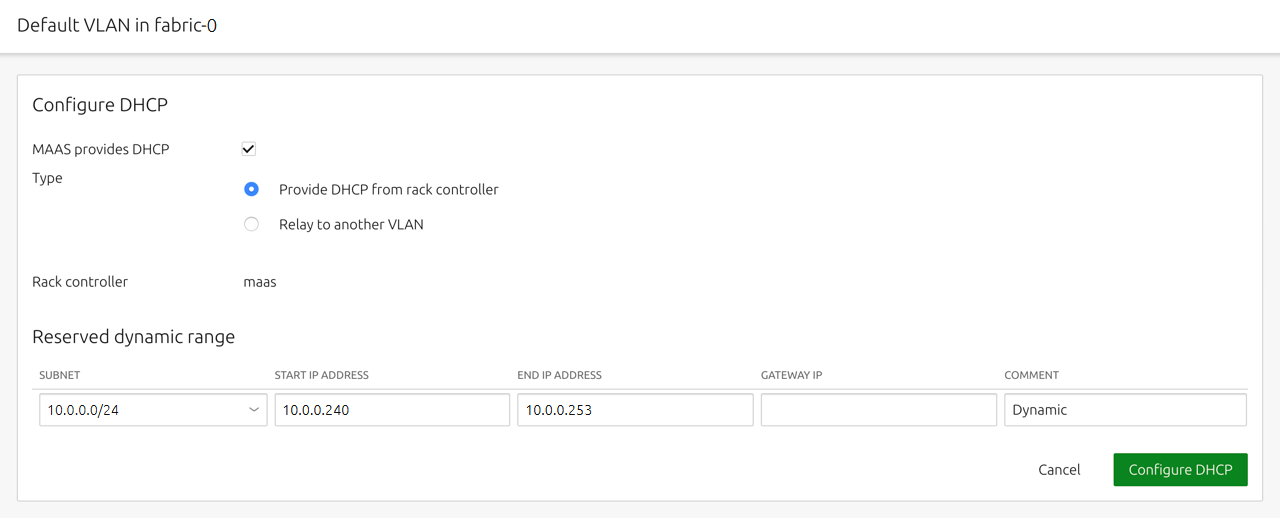
\includegraphics[width=1\linewidth]{tesi/files/immagini/maas/DHCP 240-253}
    \caption{Finestra di configurazione del DHPC.}
    \label{fig:maas_config_dhcp}
\end{figure}

\paragraph{Verifiche finali.}%\ \\%\noindent 
Ora il sistema MAAS è perfettamente funzionante.
% 
Per verificarlo basterà accedere alla schermata del controller appena configurato.
\begin{enumerate}
    \item[] 
    \begin{enumerate}
        \item Premere su "\emph{Controllers}" nel menù in alto, poi premere sul nome del controller desiderato (in questo caso \emph{maas.oscluster.unibo.it}).
        % 
        Verrà mostrata la schermata con le informazioni riguardanti il controller e lo status dei servizi in esecuzione.
        
        \item Verificare dunque che a fianco ai nomi di questi, come mostrato in \cref{fig:maas_sum_region+rack}, siano presenti le spunte verdi.
    \end{enumerate}
\end{enumerate}
% 
\begin{figure}[H]
    \centering
    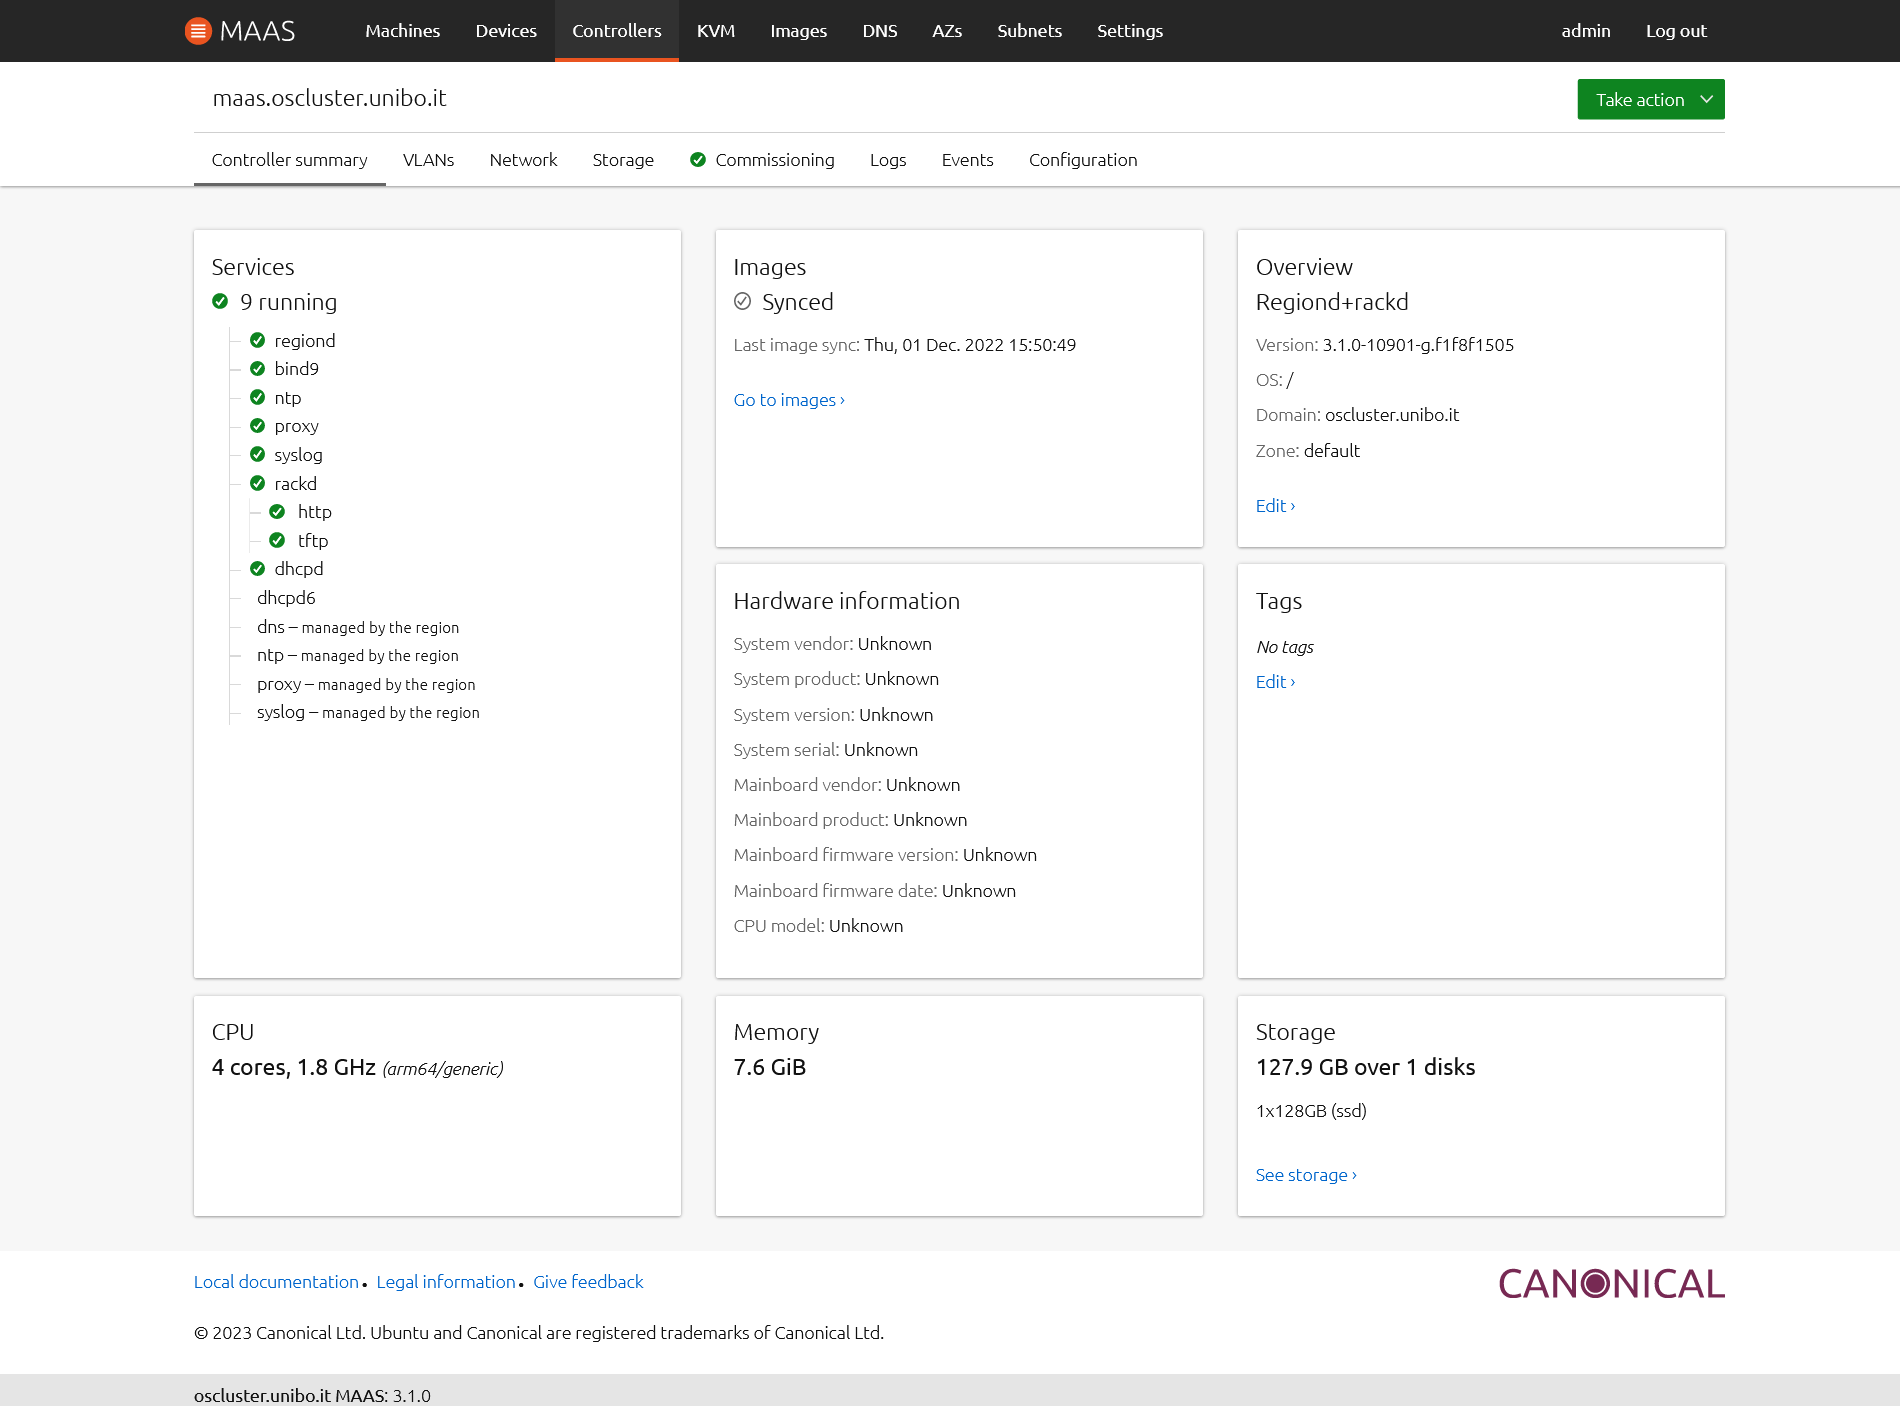
\includegraphics[width=1\linewidth]{tesi/files/immagini/maas/services_controller}
    \caption{Schermata di sintesi del region+rack controller.}
    \label{fig:maas_sum_region+rack}
\end{figure}
% 
% \paragraph{}
\bigskip
Come ultimo passaggio è consigliato verificare che le immagini selezionate nel punto \ref{itm:image_ubuntu} 
% di questa sezione
siano state scaricate correttamente.
\begin{enumerate}
    \item[] 
    \begin{enumerate}
        \item Premere su "\emph{Images}" nel menù in alto e nella schermata che comparirà.
        
        \item Verificare che le immagini scelte abbiamo come status "\emph{Synced}".
    \end{enumerate}
\end{enumerate}

\noindent
% CONFIGURAZIONE PROXY
Durante lo svolgimento del progetto sono sorti dei problemi con il Proxy HTTP integrato all'interno di MAAS.
% 
In particolare esso non permetteva alle macchine di collegarsi a internet e quindi di scaricare i software da installare e gli aggiornamenti.
% 
Dato che questa funzionalità non è strettamente necessaria per il funzionamento di tutto il sistema, è stato deciso di disabilitarla tramite la seguente procedura:
\begin{enumerate}
    \item Premere su "\textit{Settings}" nel menu in alto; in questo modo comparirà la schermata da cui è possibile modificare la configurazione del controller.
    
    \item Premere sul bottone "\textit{Proxy}" nella sottosezione "\textit{Network}".
    
    \item Selezionare la voce "\textit{Don't use a proxy}" e premere il tasto "\textit{Save}" per salvare le modifiche.
\end{enumerate}


\subsection{Aggiunta dei nodi}\label{subsubsec:maas_add_node}
Finalmente è possibile aggiungere le macchine al sistema.
% 
% Si ricordano i requisiti minimi dichiarati in AGGIUNGERE RIFERIMENTO per le singole macchine da collegare al sistema.
% 
% Inoltre 
Prima di procedere è importante verificare che nel BIOS di ciascuna macchina sia abilitata l'opzione \emph{PXE} (Preboot eXecution Environment), ovvero quella che permette il boot via rete e che sia 
in cima come priorità d'avvio.
% la prima come priorità.
% 
In caso di incertezze, consultare il manuale della scheda madre della macchina.

\bigskip
Nonostante la procedura per aggiungere i nodi possa essere eseguita simultaneamente, è consigliabile iniziare aggiungendo una macchina per volta in modo da prendere confidenza con i vari step e identificare correttamente le varie macchine.

Durante le seguenti fasi MAAS assocerà ai nodi uno status in base allo step del lifecycle; per maggiori dettagli si veda la \cref{subsubsec:maas_node}. 
% 
\begin{enumerate}
    \item \textbf{Enlist dei nodi.} Collegare la macchina alla subnet del rack controller e accenderla.
    % Accendere la macchina una volta che è stata collegata alla subnet del rack controller.
    % 
    Una volta effettuato il boot da rete, MAAS la rileva e avvia la procedura di enlist.
    % 
    A processo terminato la macchina si spegnerà e sarà possibile visualizzare il nodo appena aggiunto dall'interfaccia utente web di MAAS premendo su "\emph{Machines}" nel menù in alto. Il nodo appena aggiunto apparirà con status \emph{News}.

    \item\label{itm:powertype} \textbf{Configurazione power type.} La prima cosa da fare dopo aver aggiunto una macchina a MAAS è configurare il power type. Questo parametro indica la metodologia con la quale viene gestita l'alimentazione delle macchine. MAAS infatti ha la capacità di accendere e spegnere le macchine in autonomia nel caso queste siano predisposte (e.g. se sono dotate di una IPMI).

    È possibile configurare il power type di una macchina nel seguente modo:
    \begin{enumerate}
        \item Entrare nella schermata di visualizzazione delle macchine tramite il bottone "\emph{Machines}" nella barra di navigazione e cliccare sul nodo che si vuole configurare
        \item Aprire la scheda "\emph{Configuration}" e premere sul secondo tasto "\emph{Edit}" (quello riguardante la sezione \emph{Power configuration}).

        \item Selezionare il power type desiderato, configurarlo e al termine premere su "\emph{Save changes}" per applicare le modifiche.
    \end{enumerate}
    % 
    In questo scenario, dato che le macchine in dotazione non supportano l'avvio e lo spegnimento automatico, è stata scelta la modalità \emph{Manual}, che comporta una gestione manuale da parte dell'accensione e spegnimento delle macchine durante le varie fasi di setup.

    Per maggiori dettagli sulle varie tipologie messe a disposizione da MAAS, consultare la documentazione a riguardo \cite{maas_power_management}.

    \item \textbf{Rinominare i nodi.} È possibile rinominare i nodi, in modo tale che siano facilmente riconoscibili. Per fare questo è sufficiente entrare nella pagina di gestione del nodo, premere in alto a sinistra sul nome corrente e inserire quello nuovo; per salvare i cambiamenti è sufficiente premere invio o cliccare sul tasto "\emph{Save}".
    % 
    In questo scenario sono stati utilizzati nomi incrementativi per quanto riguarda i nodi, da \emph{node1} fino a \emph{node5}, mentre la macchina su cui verrà installato il controller Juju avrà semplicemente il nome \emph{juju}.

\end{enumerate}
% \paragraph
% \item[] \textbf{Commission.}
Una volta caricati tutti i nodi nel sistema, è possibile proseguire contemporaneamente su tutte le macchine.
\begin{enumerate}\setcounter{enumi}{3}
    \item \textbf{Commission.} MAAS ora è pronto per raccogliere le informazioni dei vari nodi.
    %
    Il tempo necessario al completamento di questa fase dipende da diversi fattori e potrebbe richiedere diversi minuti.
    \begin{enumerate}
        \item Dalla  pagina "\emph{Machines}" selezionare tutti i nodi spuntando la casella a sinistra del loro nome.
        
        \item Premere sul pulsante verde "\emph{Take action}" in alto a destra e poi premere su "\emph{Commission...}". %causa sbordo di 2 caratteri e non va a capo da solo, causando warning; vedere se aggiungere forzamento a capo prima dell'emph con \\
        
        \item A questo punto, se nel punto \ref{itm:powertype} il power type dei nodi è stato configurato su \emph{Manual}, bisognerà accendere tutti i nodi manualmente.
        % 
        Una volta completata la fase di commission, i computer si spegneranno e i nodi passeranno in stato \emph{Commissioned}.
    \end{enumerate}
    
    \item\label{itm:tag_node} \textbf{Tag dei nodi.} È possibile associare ai nodi delle etichette per facilitarne la selezione e gestione durante le fasi di installazione del cloud.
    % 
    \begin{enumerate}
        \item[] Dalla  scheda "\emph{Configuration}" di un singolo nodo, premere sul primo tasto "\emph{Edit}" e nella casella di testo "\emph{Tags}" aggiungere i tag desiderati. 
    \end{enumerate}
    % 
    In questo scenario sono stati utilizzati il tag \emph{compute} per i nodi del cloud (eccetto per il node5 al quale non è stato associato alcun tag) e il tag \emph{juju} per la macchina con il controller Juju. 

    \item\label{itm:maas_ovs_bridge} \textbf{Creazione del OvS bridge.} Come ultimo passaggio, è importate creare uno switch virtuale su ogni nodo del cloud (non la macchina juju) che verrà successivamente utilizzato per poter collegare le VM alla rete esterna.
    % 
    Per maggiori dettagli su Open vSwitch, vedasi la \cref{subsubsec:ovs}.
    \begin{enumerate}
        \item Dalla  pagina del nodo aprire la scheda "\emph{Network}", spuntare la casella a fianco al nome della rete e premere sul tasto "\emph{Create bridge}".

        \item A questo punto compare la finestra per la configurazione del OvS bridge; inserire un nome in "\emph{Bridge name}" uguale per tutti i nodi, selezionare in "\emph{Bridge type}" il valore \emph{Open vSwitch (ovs)}, inserire i parametri di rete corretti (come il  "\emph{Fabric}",  "\emph{VLAN}", "\emph{Subnet}") e in "\emph{IP mode}" selezionare \emph{Auto assign} per l'assegnamento automatico degli indirizzi IP.
    \end{enumerate}

    In \cref{fig:maas_ovs} viene mostrata la configurazione usata in questo scenario su uno dei quattro nodi del cloud;
    % 
    eccetto per il campo "\emph{MAC address}", la configurazione risulta essere la medesima per ogni nodo.
    % \end{itemize}
\end{enumerate}

\begin{figure}[H]
    \centering
    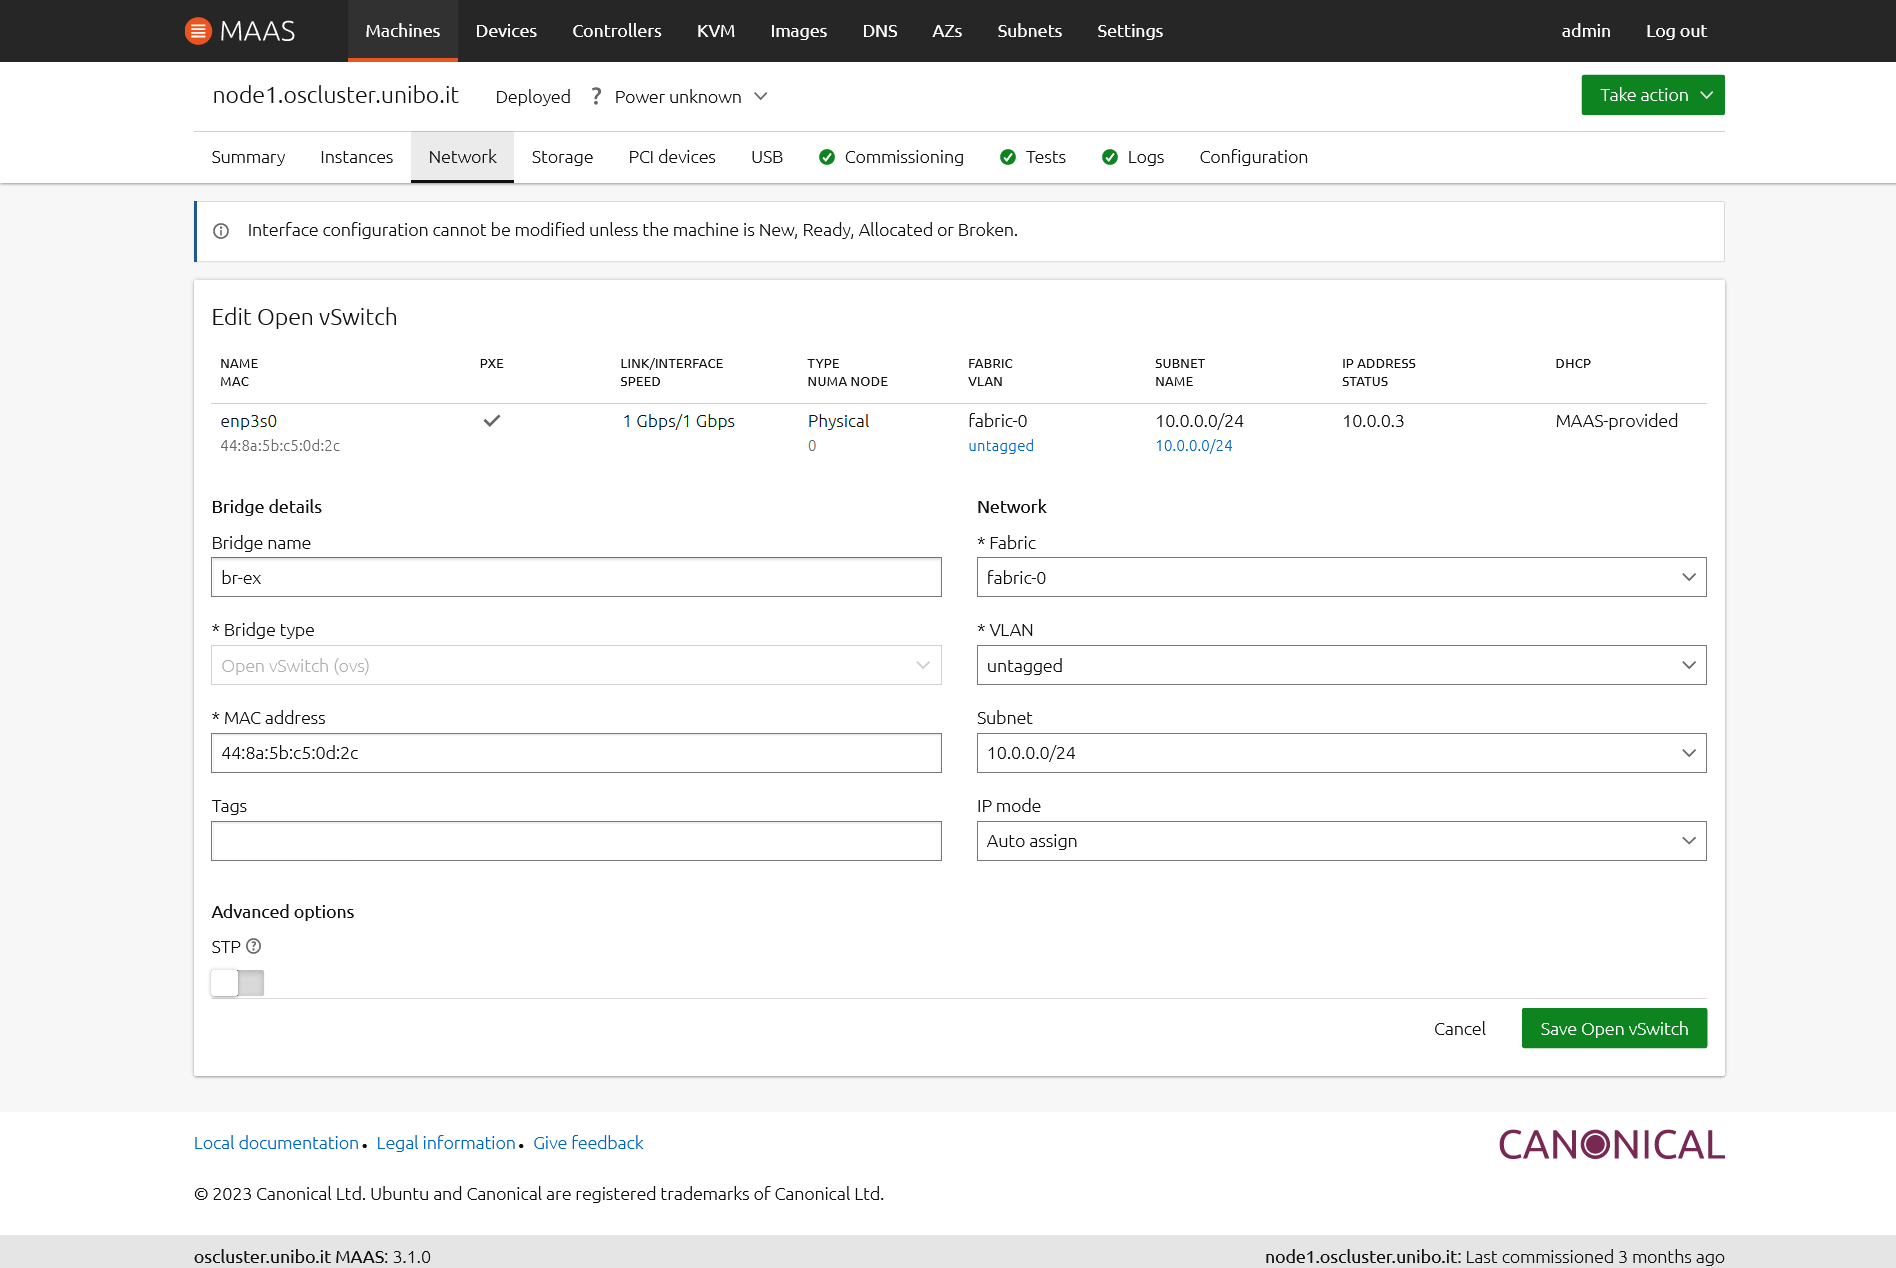
\includegraphics[width=1\linewidth]{tesi/files/immagini/maas/ovs}
    \caption{schermata di editing della configurazione Open vSwitch su un nodo.}
    \label{fig:maas_ovs}
\end{figure}


\bigskip\bigskip\noindent
L'installazione e la configurazione di MAAS è terminata.
% 
Il prossimo passo sarà quello di introdurre e installare il sistema Juju, il quale consentirà il deploy e la gestione lato software sui vari nodi. 

% 